\documentclass{article}

\usepackage{amsmath}
\usepackage{bussproofs}
\usepackage{color}
\usepackage[a4paper,margin=1in]{geometry}
\usepackage{graphicx}
\usepackage{hyperref}
\usepackage[utf8]{inputenc}
\usepackage{listings}
\usepackage{qtree}
\usepackage{tikz}

\usetikzlibrary{automata,arrows}

\lstset
{language=Haskell
,basicstyle=\footnotesize
,extendedchars=true
,literate={é}{{\'e}}1
,frame=single
}

\begin{document}
\title{Compiler Construction -- supervision 1}
\author{James Wood}
\maketitle

\begin{enumerate}
  \item
    \begin{enumerate}
      \item The operation of a DFA proceeds by taking each symbol from the input stream in order, then doing the constant time (with respect to the input) operation of lookup and transition. This gives a time complexity of $O(n)$. The DFA has no accumulating of state, so has $O(1)$ space complexity.
      \item
        \begin{lstlisting}
runDFA :: Eq o => DFA q o -> Word o -> Bool
runDFA (DFA f s as) [] = elem s as
runDFA (DFA f s as) (o : os) = runDFA (DFA f (f (s, o)) as) os
        \end{lstlisting}
      \item
        If the NFA has $q$ many states, the DFA yielded from the subset construction can have up to $2^q$ states. This means that the conversion takes $O(2^q)$ time and space in the worst case, and composing this with \texttt{runDFA} gives a time complexity of $O(2^q + n)$.
        In the worst case of simulating an NFA, the machine is in all of the $q$ states at each step of the simulation. It also transitions from each state to every other state. Deleting duplicates from the resulting state set (of size $q^2$) takes $O(q^2 \cdot \log q^2)$ (which is equivalent to $O(q^2 \cdot \log q$) time (assuming that the state labels are orderable). This gives a time complexity of $O(n \cdot q^2 \cdot \log q)$.
        Loosely, converting to a DFA and then simulating the DFA is faster when the input is large and the NFA is small. It is also better if the same NFA is to be used on many different inputs, because the DFA can be computed once and saved for later.
      \item The algorithm recomputes the state of the finite automaton corresponding to each regular expression each time it checks the buffer against a rule.
      \item Instead, it would be more time-efficient to save the state of the finite automaton for each regular expression, and advance each as symbols arrive from the input stream. Assuming that DFAs are available for the regular expressions, this would give a time complexity of $O(r \cdot n)$, where $r$ is the number of rules and $n$ is the length of the input.
    \end{enumerate}
  \item
    \begin{enumerate}
      \item
        \begin{enumerate}
          \item Yes:
            \begin{prooftree}
              \AxiomC{}
              \RightLabel{\scriptsize $X ::= \varepsilon$}\UnaryInfC{$\varepsilon$ matches $X$}
              \RightLabel{\scriptsize $S ::= X$}\UnaryInfC{$\varepsilon$ matches $S$}
              \UnaryInfC{$\varepsilon \in L(G)$}
            \end{prooftree}
          \item No. The only words starting with $a$ end with $b$ (having matched $X$).
          \item Yes:
            \begin{prooftree}
              \AxiomC{}
              \RightLabel{\scriptsize $Z ::= \varepsilon$}\UnaryInfC{$\varepsilon$ matches $Z$}
              \RightLabel{\scriptsize $S ::= cZ$}\UnaryInfC{$c$ matches $S$}
              \UnaryInfC{$c \in L(G)$}
            \end{prooftree}
          \item Yes:
            \begin{prooftree}
              \AxiomC{}
              \RightLabel{\scriptsize $X ::= \varepsilon$}\UnaryInfC{$\varepsilon$ matches $X$}
              \RightLabel{\scriptsize $X ::= aXb$}\UnaryInfC{$ab$ matches $X$}
              \RightLabel{\scriptsize $S ::= X$}\UnaryInfC{$ab$ matches $S$}
              \UnaryInfC{$ab \in L(G)$}
            \end{prooftree}
          \item No. All words starting with $b$ are $bbc$, having matched $Y$.
          \item Yes:
            \begin{prooftree}
              \AxiomC{}
              \RightLabel{\scriptsize $Y ::= bbc$}\UnaryInfC{$bbc$ matches $Y$}
              \RightLabel{\scriptsize $S ::= Y$}\UnaryInfC{$bbc$ matches $S$}
              \UnaryInfC{$bbc \in L(G)$}
            \end{prooftree}
          \item No. All words ending with $d$ end with $dd$, having matched $Z$.
          \item Yes:
            \begin{prooftree}
              \AxiomC{}
              \RightLabel{\scriptsize $Z ::= \varepsilon$}\UnaryInfC{$\varepsilon$ matches $Z$}
              \RightLabel{\scriptsize $Z ::= cZdd$}\UnaryInfC{$cdd$ matches $Z$}
              \RightLabel{\scriptsize $S ::= cZ$}\UnaryInfC{$ccdd$ matches $S$}
              \UnaryInfC{$ccdd \in L(G)$}
            \end{prooftree}
          \item No. All words beginning with $c$ end with $d$, having matched $Z$.
          \item No. The only way to match the initial $c$s is via $Z$, and the closest matches are $ccdd$ and $cccdddd$.
          \item Yes:
            \begin{prooftree}
              \AxiomC{}
              \RightLabel{\scriptsize $X ::= \varepsilon$}\UnaryInfC{$\varepsilon$ matches $X$}
              \RightLabel{\scriptsize $X ::= aXb$}\UnaryInfC{$ab$ matches $X$}
              \RightLabel{\scriptsize $X ::= aXb$}\UnaryInfC{$aabb$ matches $X$}
              \RightLabel{\scriptsize $X ::= aXb$}\UnaryInfC{$aaabbb$ matches $X$}
              \RightLabel{\scriptsize $S ::= X$}\UnaryInfC{$aaabbb$ matches $S$}
              \UnaryInfC{$aaabbb \in L(G)$}
            \end{prooftree}
        \end{enumerate}
      \item The leftmost derivation is the derivation in which any rules are instantiated by having as much of the string as possible matched by non-terminal symbols to the left of the rule's body. The rightmost derivation is defined similarly. The leftmost derivation can be parsed using recursive descent parsing (after transforming the grammar to avoid left recursion). The rightmost derivation can be parsed using shift-reduce parsing.
      \item Take the following grammar:
        \begin{align*}
          E & ::= E - E \mid 1
        \end{align*}
        This can parse the expression $1 - 1 - 1$ as either of the following:

        \Tree[.$E$ [.$E$ [.$1$ ] ] [.$-$ ] [.$E$ [.$E$ [.$1$ ] ] [$-$ ] [.$E$ [.$1$ ] ] ] ]
        \Tree[.$E$ [.$E$ [.$E$ [.$1$ ] ] [$-$ ] [.$E$ [.$1$ ] ] ] [.$-$ ] [.$E$ [.$1$ ] ] ]
      \item
        \begin{align*}
          E & ::= E + E' \mid E - E' \mid E' \\
          E' & ::= E'! \mid \left(E'\right) \mid a \mid b \mid c
        \end{align*}
    \end{enumerate}
  \item
    \begin{enumerate}
      \item
        \begin{itemize}
          \item $S \to {} \cdot aABe$
          \item $S \to a \cdot ABe$
          \item $S \to aA \cdot Be$
          \item $S \to aAB \cdot e$
          \item $S \to aABe \cdot {}$ -- complete
        \end{itemize}
      \item
        \begin{enumerate}
          \item The handle of $aABe$ is $aABe$ ($\delta := \varepsilon$, $A := S$, $w := \varepsilon$).
          \item The handle of $aAde$ is $d$ ($\delta := aA$, $A := B$, $w := e$).
          \item The handle of $abcAde$ is $bcA$ ($\delta := a$, $A := A$, $w := de$).
        \end{enumerate}
      \item
        \begin{enumerate}
          \item For $aABe$: $\varepsilon$, $a$, $aA$, $aAB$, $aABe$.
          \item For $aAde$: $\varepsilon$, $a$, $aA$, $aAd$.
          \item For $abcAde$: $\varepsilon$, $a$, $ab$, $abc$, $abcA$.
        \end{enumerate}
      \item
        \begin{enumerate}
          \item For $aABe$:
            \begin{itemize}
              \item $a$ has valid item $S \to a \cdot ABe$.
              \item $aA$ has valid item $S \to aA \cdot Be$.
              \item $aAB$ has valid item $S \to aAB \cdot e$.
              \item $aABe$ has valid item $S \to aABe \cdot {}$.
            \end{itemize}
          \item For $aAde$:
            \begin{itemize}
              \item $a$ and $aA$ have valid item $B \to {} \cdot d$.
              \item $aAd$ has valid item $B \to d \cdot {}$.
            \end{itemize}
          \item For $abcAde$:
            \begin{itemize}
              \item $a$ has valid item $A \to {} \cdot bcA$.
              \item $ab$ has valid item $A \to b \cdot cA$.
              \item $abc$ has valid item $A \to bc \cdot A$.
              \item $abcA$ has valid item $A \to bcA \cdot {}$.
            \end{itemize}
        \end{enumerate}
      \item This:

        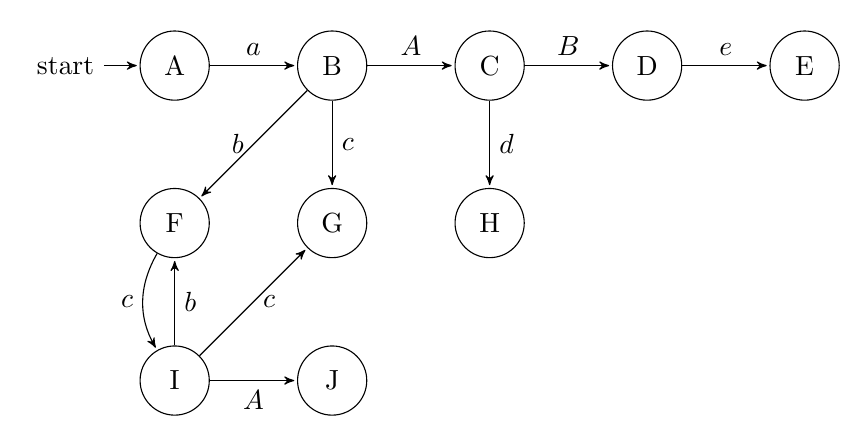
\begin{tikzpicture}[>=stealth',shorten >=1pt,auto,node distance=2cm, transform shape,every node/.style={align=center}]
          \node[initial,state] (A) {A};
          \node[state] (B) [right of=A] {B};
          \node[state] (C) [right of=B] {C};
          \node[state] (D) [right of=C] {D};
          \node[state] (E) [right of=D] {E};
          \node[state] (F) [below of=A] {F};
          \node[state] (G) [below of=B] {G};
          \node[state] (H) [below of=C] {H};
          \node[state] (I) [below of=F] {I};
          \node[state] (J) [right of=I] {J};

          \path[->]
            (A) edge node [above] {$a$} (B)
            (B) edge node [above] {$A$} (C)
            (C) edge node [above] {$B$} (D)
            (D) edge node [above] {$e$} (E)
            (B) edge node [left] {$b$} (F)
            (F) edge [bend right] node [left] {$c$} (I)
            (I) edge node [right] {$b$} (F)
            (I) edge node [below] {$A$} (J)
            (B) edge node [right] {$c$} (G)
            (I) edge node [right] {$c$} (G)
            (C) edge node [right] {$d$} (H)
            ;
        \end{tikzpicture}

        \begin{tabular}{r | l}
          State & Items \\
          \hline
          A & $S \to {} \cdot aABe$ \\
          B & $S \to a \cdot ABe$; $A \to {} \cdot bcA$; $A \to {} \cdot c$ \\
          C & $S \to aA \cdot Be$; $B \to {} \cdot d$ \\
          D & $S \to aAB \cdot e$ \\
          E & $S \to aABe \cdot {}$ \\
          F & $A \to b \cdot cA$ \\
          G & $A \to c \cdot {}$ \\
          H & $B \to d \cdot {}$ \\
          I & $A \to bc \cdot A$; $A \to {} \cdot bcA$; $A \to {} \cdot c$ \\
          J & $A \to bcA \cdot {}$ \\
        \end{tabular}
      \item
        \begin{tabular}[t]{l | l | l}
          Stack & Input stream & Next operation \\
          \hline
          A & $abccde$ & shift B \\
          A $a$ B & $bccde$ & shift F \\
          A $a$ B $b$ F & $ccde$ & shift I \\
          A $a$ B $b$ F $c$ I & $cde$ & shift G \\
          A $a$ B $b$ F $c$ I $c$ G & $de$ & reduce $A \to c$, goto J \\
          A $a$ B $b$ F $c$ I $A$ J & $de$ & reduce $A \to bcA$, goto C \\
          A $a$ B $A$ C & $de$ & shift H \\
          A $a$ B $A$ C $d$ H & $e$ & reduce $B \to d$, goto D \\
          A $a$ B $A$ C $B$ D & $e$ & shift E \\
          A $a$ B $A$ C $B$ D $e$ E & & accept $S \to aABe$ \\
        \end{tabular}
      \item The stack grows linearly until the parser reaches $d$, at which point there are many consecutive reductions. This happens because of the rule $A \to bcA$, which is recursive in a non-initial position. In this case, it is recursive in the final position, so it should be possible to do something similar to tail call elimination. Specifically, whenever state I is reached and $b$ is found, we can collapse the preceeding $bc$ (somewhere keeping count of how many of these we have encountered) and continue from state F.
      \item Lookahead allows a parser to know something about $w$ before committing to using $A \to \alpha$. For the first problem, we get to know something about $w'$, which may distinguish it from $w$. For the second problem, we are putting constraints against what items are valid in a given state. For the third problem, lookahead allows us to test (to the given extent) whether there are handles of $\gamma w$ containing characters of $w$.
      \item DFAs and parse tables for LR($k$) grammars can become very large. Converting the DFA into an LALR($k$) DFA reduces its size significantly by merging states with matching items but different lookahead tokens. This gives a refinement on LR($0$) without introducing extra states.
    \end{enumerate}
\end{enumerate}

\section*{Practical exercises}
See the commit history of \url{https://github.com/laMudri/compconstr-code}.

\end{document}
